%\providecommand{\main}{..}
%\documentclass[\main/main.tex]{subfiles}


\begin{document}


\section{Descriptive statistics}

\subsection{Sample size}
After the data cleaning, we are left with the following sample size (all waves together):

\begin{table}[H]
\begin{center}
\begin{tabular}{llrr}
\toprule
{} & \textbf{Country} &    \textbf{Male}    &  \textbf{Female}      \\
\midrule
 & Austria &   5907 &   7871 \\
        & Belgium &   9415 &  11241 \\
        & Denmark &   6174 &   7060 \\
        & France &   7348 &   9414 \\
        & Germany &   6686 &   7494 \\
        & Italy &   8325 &   9807 \\
        & Spain &   8391 &  10130 \\
        & Sweden &   6625 &   7555 \\
        & Switzerland &   4437 &   5123 \\
\bottomrule
\end{tabular}
\captionsetup{justification=centering}
\caption{Sample size by country \\ \textit{Source:} re-produced from EASYSHARE}
\end{center}
\end{table}

\subsection{Disability status}
Figure \ref{fig:disability_True} describes the distribution of disability status by gender and income decile. We consider the whole sample, i.e. individuals aged 50 years old or older, living in any of the nine selected countries and interviewed in any of the five waves. From this simple descriptive chart, one can easily notice that the majority of respondents reports being in a healthy status but, at the same time, there are some remarkable differences.\\




\begin{figure}[H]
    \centering \textbf{Healthy and disabled status}\par\medskip
    \begin{minipage}{.5\textwidth}
        \centering
        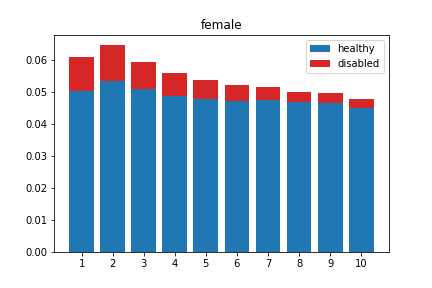
\includegraphics[scale=.5]{images/disability_female.png}
    \end{minipage}%
   \begin{minipage}{.5\textwidth}
        \centering 
        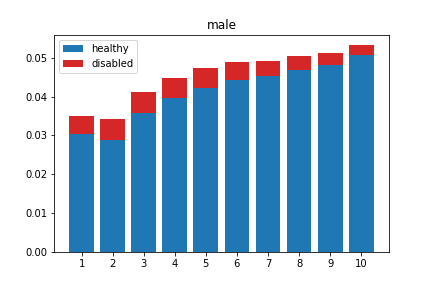
\includegraphics[scale=.5]{images/disability_male.png}
    \end{minipage}
    \captionsetup{justification=centering}
    \caption{Percentage of individuals by gender, income, and disability status \\ \textit{Source:} re-produced from EASYSHARE}
    \label{fig:disability_True_all}
\end{figure}

\begin{figure}[H]
    \centering
    \begin{minipage}{.5\textwidth}
        \centering
        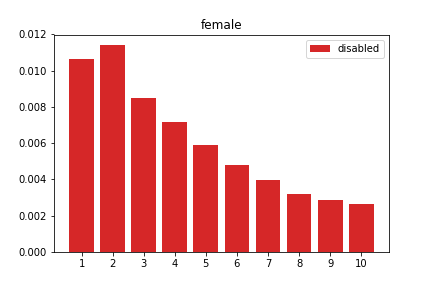
\includegraphics[scale=.5]{images/disability_only_female.png}
    \end{minipage}%
   \begin{minipage}{.5\textwidth}
        \centering
        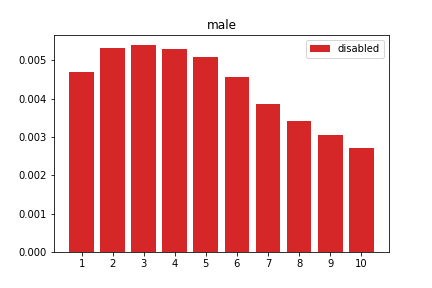
\includegraphics[scale=.5]{images/disability_only_male.png}
    \end{minipage}
    \captionsetup{justification=centering}
    \caption{Percentage of disabled individuals by gender and income \\ \textit{Source:} re-produced from EASYSHARE}
    \label{fig:disability_True}
\end{figure}

First of all, income is not uniformly distributed across gender: there are more females in the lowest income percentiles than in the highest ones. For instance, around 6\% of the survey participants are female in the $1^{st}$ income percentile as opposed to 5\% in the $10^{th}$ income percentile. Conversely, men tend to have a higher income: 3.5\% of the participants are male in the $1^{st}$ income percentile while 5.5\% are in the $10^{th}$ income percentile. \\

Moreover, there appears to be a higher prevalence of disability status in the female population than in male one. For example, the peak of disability for female participants is around 1.2\% (in the $2^{nd}$ income percentile), while for men it is around 0.55 \% (in the $3^{rd}$ income percentile).\\

Finally, disability status appears to be negatively associated with income, with respondents in the higher income percentiles being less likely to report a disability. However, these differences across groups appear more evident for females than for men, especially with respect to first six income percentiles.


\subsection{Age distribution}

To explore the data set more thoroughly, we plotted the fitted distribution of the age variable for each income percentile and country. Figure \ref{fig:age_distr_germany} presents the plot that characterises the German sample and which can be considered a good representative example. As we can see, younger people (i.e. between 50 and 70 years old) are more likely to belong to the highest income groups. This is an expected result as people in this age interval are usually in the labour market earning a full salary, while older people are more likely to receive a pension income, which is typically lower.\\
However, the fact that the age distribution differs by income group should not bias our estimate, even though it might produce heterogeneity in the width of the confidence interval estimated for our prevalence data.  \\

For instance, considering the $10^{th}$ income decile and computing prevalence data for disability (i.e. the proportion of disabled in a given age group over total population in that age groups), the estimates for the younger age groups are likely to be more precise than the ones of older ages, since we observe more data in the first group and fewer individuals in the latter. The opposite will hold true for lower income groups, thus producing heterogeneity in the width of the confidence interval.



\begin{figure}[H]
        \centering
        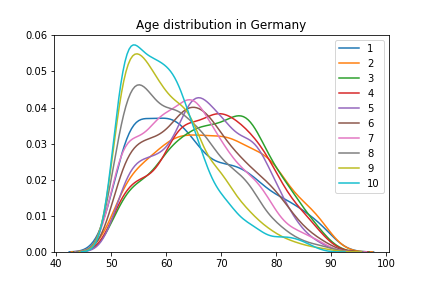
\includegraphics[scale=.5]{images/Age_distribution_in_Germany.png}
            \captionsetup{justification=centering}
    \caption{Fitted distribution of age by income decile, Germany \\ \textit{Source:} re-produced from EASYSHARE}
    \label{fig:age_distr_germany}
\end{figure}



\end{document}